\section{Data}
\label{sec:chromium-data}

\subsection{Definitions}

Some of our definitions are slightly different from the ones used by previous work since Chromium has its specific continuous integration setup. To make things clear, we define the elements we will discuss in this section.  
In the scope of \emph{a single build}, we employ the following definitions: 
\begin{itemize}
    \item \textbf{Fault-revealing test}: A test that consistently failed after reruns in the same build, revealing a regression fault.
    \item \textbf{Flaky test}: A test that failed once or more and then passed after reruns in the same build. 
    \item\textbf{Flaky failure}: A test failure caused by a flaky test.
    \item\textbf{Fault-triggering failure}: A test failure caused by a fault-revealing test.\\
\end{itemize}


\subsection{Data Collection}

To perform our study, we collected test execution data from 10,000 consecutive builds completed by the Linux Tester by querying the LuCI API. This represents a period of time of about 9 months taken between March 2022 and December 2022. 

Table ~\ref{table:infoRuns} summarises the list of information extracted and computed for all tests executed in all builds. The \textsc{buildId} corresponds to the build in which tests were executed. \textsc{runDuration} is the execution time spent to run the test. \textsc{runStatus} gives information about the run result (\eg passing, failing, and skipped) and \textsc{runTagStatus} returns more precise information about the result of a run depending on the type of test or test suite (\eg timeout and failure on exit). We retrieved information about the tests' source code by querying Google Git~\footnote{https://chromium.googlesource.com/chromium/src/+/HEAD/}. As builds often handle several commits, we select the revision corresponding to the head of the blame list: the one on which tests were executed. The \textsc{testSuite} is simply the name of the test suite the test belongs to and \textsc{testId} is a unique identifier for a test composed of the test suite and the test name (the same test name can be present in different test suites).

All the scripts used to collect the data alongside the created dataset are available in our replication package.

\begin{table}[!ht]
\centering
\caption{Description of our features. Column \textit{Feature Name} specifies the identifiers used in our dataset, while Column \textit{Feature Description} details the features}
\label{table:infoRuns}
\begin{tabular}{ l | l } 
\toprule
\textbf{Feature Name} & \textbf{Feature Description} \\
\midrule
buildId & The build number associated \\
{} & with the test execution \\
\midrule
flakeRate & The flake rate of the test over the last\\  
{} & 35 builds \\
\midrule
runDuration & The time spent for this test execution \\
\midrule
runStatus & ABORT\\ {} & FAIL\\ {} & PASS\\ {} & CRASH\\ {} & SKIP \\
\midrule
\multirow[t]{9}{*}{runTagStatus} & CRASH\\ {} & PASS\\ {} & FAIL\\ {} & TIMEOUT\\ {} & SUCCESS \\
{} & FAILURE\\ {} & FAILURE\_ON\_EXIT\\ {} & NOTRUN\\ {} & SKIP\\ {} & UNKNOWN \\
\midrule
testSource & The test source code \\
\midrule
testSuite & The test suite the test belongs to \\
\midrule
testId & The test name \\
\bottomrule
\end{tabular}
\end{table}

% Table: Data collected from the Chromium CI
% Script: infoDataset.py
\begin{table*}[ht]
\centering
\caption{Data collected from the Chromium CI. We used the \textit{Linux Tests} tester, with \textit{10,000} Builds mined over \textit{nine} months. We extracted Passing, Flaky and Fault-revealing tests and their associated Flaky and Fault-triggering Failures.}
\label{table:infoDataset}
\resizebox{\textwidth}{!}{\begin{tabular}{ l | c | c c | c c c | c c } 
\toprule
\multirow{2}{*}{\textbf{Tester}} & \multirow{2}{*}{\textbf{Nb of Builds}} & \multicolumn{2}{c|}{\textbf{Period of Time}} & \multicolumn{3}{c|}{\textbf{Number of Tests}} & \multicolumn{2}{c}{\textbf{Number of Failures}} \\
{} & {} & \textbf{From} & \textbf{To} & \textbf{Passing} & \textbf{Flaky} & \textbf{Fault-revealing} & \textbf{Flaky} & \textbf{Fault-triggering} \\
\midrule 
Linux Tests & 10,000 & Mar 2, 2022 & Dec 1, 2022 & 198,273 & 23,374 & 2,343  & 1,833,831 & 17,171 \\
\bottomrule
\end{tabular}}
\end{table*}

\subsection{Computing the Flake Rate}
\label{sec:testHistory}

The historical sequence of test results is a valuable piece of information commonly used in software testing at scale~\cite{LeongSPTM19,Kowalczyk2020}. We analyse the history of fault-revealing tests and flaky tests by relying on their \textsf{flakeRate}.

This means that for a test $t$ failing (due to flaky or fault-triggering failure) in a build $b_{n}$, we analyse all the builds from a time window $w$ (\ie from $b_{n-w}$ to $b_{n-1})$ to calculate its flake rate as follows: \\

\noindent\begin{minipage}{\linewidth}
\begin{equation}
  flakeRate(t,n) = \frac{ \sum_{x=n-w}^{n-1} flake(t,x) } {w}
\end{equation}
\end{minipage}%
\\

where $flake(t,x) = 1$ if the test $t$ flaked in the build $b_{x}$ and 0 otherwise.
This metric allows us to understand if the flakiness history of a test can help in the flakiness prediction tasks.
The test execution history (\aka heartbeat) has been used in multiple studies (especially industrial ones~\cite{Kowalczyk2020,LeongSPTM19}) to detect flaky tests.
These studies assume that many flaky tests have distinguishable failure patterns over builds and hence can be detected by observing their history.
We check whether this assumption also holds in the case of Chromium.

\begin{figure}[ht]
  \centering
    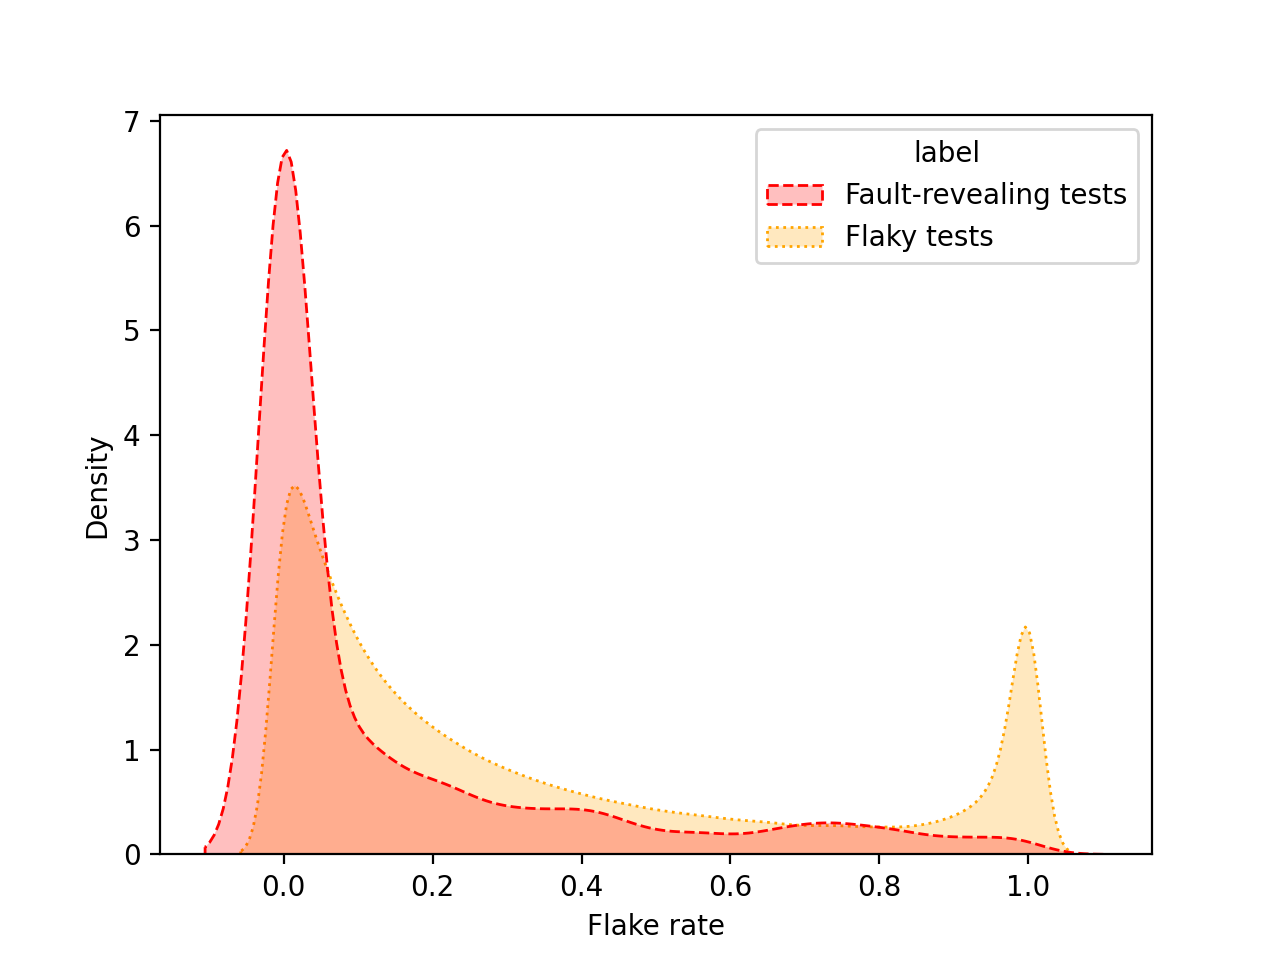
\includegraphics[width=0.8\textwidth]{figures/chromium/densityFlakeRate.png}
    \caption{Flake rate (\textit{x-axis}) for \textcolor{orange}{Flaky} and \textcolor{red}{Fault-revealing tests}. Density (\textit{y-axis}) is the probability density function. The area under curves integrates to one. Many flaky tests are always flaky in their previous builds. A majority of fault-revealing tests have no history of flakiness at all.}
    \label{fig:kdeRates}
\end{figure}

To illustrate the flake rate differences between flaky and fault-revealing tests, we plot the flake rate for both test categories in Figure~\ref{fig:kdeRates}. The flake rate is computed using a window of 35 builds. To set this time window, we checked the number of flaky tests having a $flakeRate() = 0$ for build windows ranging from 0 to 40 builds with a step of 5. We observed a convergence at size 35, meaning that higher numbers of builds do not provide additional information.

In the majority of cases, flaky tests have a history of flakiness: the percentage of flaky tests having a $flakeRate() > 0$ is in fact $87.9\%$. Furthermore, we see a pike for $flakeRate() == 1$, 9.5\% of flaky tests were always flaky in their 35 previous builds. 
Still, there is a non-negligible amount (45.3\%) of fault-revealing tests that were flaky at least once in previous builds considered: with a $flakeRate() > 0$.
From these observations, we may suggest that the \textsf{flakeRate()} can be used to detect flakiness.
Nevertheless, there is still an important overlap between the history of flaky tests and fault-revealing tests. 

